\documentclass[journal]{IEEEtran}

\usepackage{subfigure}
\usepackage{setspace}
\usepackage[labelsep=period]{caption}  
\usepackage[british]{babel} 
\usepackage{amsfonts,amsmath,bm,bbm}
\usepackage{hyperref} 
\usepackage{graphicx,xurl}
\usepackage{rotating}
\usepackage{todonotes}
\usepackage{lipsum}
\usepackage{xcolor} 
\usepackage{tikz}
\usepackage{ifthen}
\usepackage{color}
\usepackage{multicol}
\usepackage{float}

\renewcommand{\Bbb}{\mathbb}

% Author Orchid ID: enter ID or remove command
%\newcommand{\orcidauthorA}{0000-0001-9647-0506} 
%\newcommand{\orcidauthorB}{0000-0002-8002-5341} 
%\newcommand{\orcidauthorC}{0000-0002-1288-2528} 
%\newcommand{\orcidauthorD}{0000-0003-4523-6466}

\newdimen\HilbertLastX
\newdimen\HilbertLastY
\newcounter{HilbertOrder}

\def\DrawToNext#1#2{%
   \advance \HilbertLastX by #1
   \advance \HilbertLastY by #2
   \pgfpathlineto{\pgfqpoint{\HilbertLastX}{\HilbertLastY}}
}

% \Hilbert[right_x,right_y,left_x,left_x,up_x,up_y,down_x,down_y]
\def\Hilbert[#1,#2,#3,#4,#5,#6,#7,#8] {
  \ifnum\value{HilbertOrder} > 0%
     \addtocounter{HilbertOrder}{-1}
     \Hilbert[#5,#6,#7,#8,#1,#2,#3,#4]
     \DrawToNext {#1} {#2}
     \Hilbert[#1,#2,#3,#4,#5,#6,#7,#8]
     \DrawToNext {#5} {#6}
     \Hilbert[#1,#2,#3,#4,#5,#6,#7,#8]
     \DrawToNext {#3} {#4}
     \Hilbert[#7,#8,#5,#6,#3,#4,#1,#2]
     \addtocounter{HilbertOrder}{1}
  \fi
}

% \hilbert((x,y),order)
\def\hilbert((#1,#2),#3){%
   \advance \HilbertLastX by #1
   \advance \HilbertLastY by #2
   \pgfpathmoveto{\pgfqpoint{\HilbertLastX}{\HilbertLastY}}
   \setcounter{HilbertOrder}{#3}
   \Hilbert[1mm,0mm,-1mm,0mm,0mm,1mm,0mm,-1mm]
   \pgfusepath{stroke}%
}

% correct bad hyphenation here
\hyphenation{op-tical net-works semi-conduc-tor}


\begin{document}

\title{Analysis and Classification of SAR Textures using Information Theory}

\author{Eduarda~T.~C.~Chagas,%\orcidA{}
        Alejandro~C.~Frery, %\orcidB{}
        \IEEEmembership{IEEE~Senior~Member,}
        Osvaldo~A.~Rosso, %\orcidC{}
        and~Heitor~S.~Ramos %\orcidD{}
        
        \thanks{E. T. C. and H. S. Ramos are with Departamento de Ci\^encia da Computa\c c\~ao, Universidade Federal de Minas Gerais, Belo Horizonte, Minas Gerais, Brazil (e-mail: eduarda.chagas@dcc.ufmg.br, ramosh@dcc.ufmg.br).}
        \thanks{A. C. Frery is with Laborat\'orio de Computa\c c\~ao Cient\'ifica e An\'alise Num\'erica -- LaCCAN, Universidade Federal de Alagoas, Brasil; (e-mail: acfrery@laccan.ufal.br)}
        \thanks{O. A. Rosso is with Instituto de F\'isica, Universidade Federal de Alagoas, Brasil (e-mail: oarosso@if.ufal.br)}
        \thanks{Manuscript received XX YY, 20ZZ; revised WW UU, 20VV.}}


\markboth{IEEE JOURNAL OF SELECTED TOPICS IN APPLIED EARTH OBSERVATIONS AND REMOTE SENSING}
%\markboth{IEEE JOURNAL OF SELECTED TOPICS IN APPLIED EARTH OBSERVATIONS AND REMOTE SENSING,~Vol.~13, No.~9, September~2014}%
{Shell \MakeLowercase{\textit{et al.}}: Bare Demo of IEEEtran.cls for Journals}

\maketitle

\begin{abstract}
   We propose a new technique for SAR image texture analysis and classification based on the Bandt-Pompe symbolization.
   It consists of
   (i)~linearize a 2-D patch of the image using the Hilbert-Peano curve,
   (ii)~build an Ordinal Pattern Transition Graph that considers the data amplitude encoded into the weight of the edges;
   (iii)~obtain a probability distribution function derived from this graph;
   (iv)~compute Information Theory descriptors (Permutation Entropy and Statistical Complexity) from this distribution, and use them as features to feed a classifier.
   The ordinal pattern graph we propose considers that the weight of the edges is related to the absolute difference of observations, which encodes the information about the data amplitude. This modification takes into account the scattering properties of the target and leads to a reasonable characterization of several types of textures.
   Experiments with data from Munich urban areas, Guatemala forest regions, and Cape Canaveral ocean samples demonstrate the effectiveness of our technique, which achieves satisfactory levels of separability.
   The two descriptors chosen in this work are easy and quick to calculate and are used as input for a  k-nearest neighbor classifier.
   Experiments show that this technique presents results similar to state-of-the-art techniques that require a much larger number of features and consequently require a higher computational cost.
\end{abstract}

\begin{IEEEkeywords}
Synthetic Aperture Radar (SAR), Time-series, Terrain ,Classification, Ordinal Patterns Transition Graphs.
\end{IEEEkeywords}

\IEEEpeerreviewmaketitle

\section{Introduction}

\IEEEPARstart{L}{and} cover maps of remote sensing data are the most used earth observation (OE) products of remote sensing applications. In this context, the use of SAR (Synthetic Aperture Radar) systems, which can provide high-resolution images in all weather and day-night conditions, is particularly promising.
Surface classification and land use are among the most critical applications of SAR images, and the development of efficient strategies to cope with this problem is an ongoing research topic~\cite{Pottier2004Unsupervised}, for which supervised and unsupervised classification algorithms have been proposed~\cite{han2020unsupervised,huang2020classification,xie2020polsar}.
Such methods can be generally divided into two categories: methods based on SAR image statistical information and methods based on textural information~\cite{guan2019covariance}.

Extraction and analysis of characteristics are crucial steps in the classification of regions, along with additional information and previous knowledge about the scene, the sensor, and the acquisition conditions.
The study of SAR textures reveals more information about the target under analysis, being extremely important to characterize it quantitatively.

The tonal values in a synthetic aperture radar (SAR) image represent point measurements of the backscatter coefficient and are related to radar wavelength and interaction with elements in the scene.
Through textural information, we acquire data from the spatial distribution of gray levels of the image and statistics about it.

The study of textures in remote sensing presents some peculiarities concerning the analysis of isolated patterns since the texture represents only part of the scene under investigation, and it is necessary to consider micro and macro-textural structures of the image during the characterization.
However, texture analysis in SAR images provides essential information in addition to image gray levels or backscatter values and demonstrates improvements in accuracy in surface characterization due to the structural properties of different regions.
 
SAR textures can be studied following two approaches, analyzing the marginal properties of the data and observing their spatial structure~\cite{numbisi2018multi}.
In this work, we focus on the second.

In the existing literature, resource extraction followed by classification have often been applied, becoming the two significant steps that formed the basis for the analysis of satellite images~\cite{feng2014amplitude}.
Different measures of texture proved to be essential for satellite images to derive the spatial contour of the surface, the arrangement and other varieties of soil properties.

The most widely used approach to obtain textural features from SAR imagery is through co-occurrence matrices and Haralick's descriptors~\cite{yu2019detection}.
In \cite{radford2018geological},  the application of machine learning for geological mapping in remote and inaccessible localities is validated using  Random Forests and textural information derived from gray-level co-occurrence matrices obtaining an accuracy of $\approx90\%$ even when using limited training data ($\approx0.15\%$ of total data). 
In \cite{hagensieker2018evaluation}, the synergistic contribution of multi-temporal L-, C-, and X-band data to tropical land cover mapping is evaluated, comparing classification outcomes of ALOS-2~\cite{kankaku2013alos}, RADARSAT-2~\cite{morena2004introduction}, and TerraSAR-X~\cite{breit2009terrasar} 
%\todo[inline]{Incluir referências para os datasets}
%DONE
datasets for a study site in the Brazilian Amazon using a wrapper approach. 
The wrapper utilizes the gray-level co-occurrence matrix (GLCM)
%\todo{esse termo é novo, tem que itnroduzir o acrônimo}
%DONE
texture information and a  Random Forest classifier to estimate scene importance. 
In \cite{storie2018urban}, an open-source workflow for detecting and delineating the urban-rural boundary is proposed, using Sentinel-1a SAR data.
A combination of GLCM information and a k-means classifier is used to produce a three-category map that distinguishes urban from rural areas. 
Other approaches include the Fourier power  spectrum~\cite{Florindo2012Fractal}, and random fields~\cite{zhu2016antarctic}.

In our approach, we opt to analyze the 1-D signals resulting from the linearization of the image samples, using non-parametric time series analysis techniques.
By selecting this line of research, we reduce the dimensionality of the data and map the spatial dependence of the pixels to a temporal correlation of a data sequence.
Next, we extract a probability distribution from the ordinal patterns of a new transition graph, herein proposed,  which can discriminate different levels of amplitude, and we use well-known features borrowed from the information theory field to classify texture patches.
	
The main contribution of this work is the proposal of a new set of features for characterization and classification of SAR textures, based on a modification of the current ordinal patterns transition graph, incorporating important time-series information.
Our proposal, hereinafter referred to as Weighted Amplitude Transition Graph (WATG), incorporates the absolute difference between the observations, weighting them in the calculation of the final value of their probabilities.
Experiments performed on SAR image textures indicate that this approach preserves essential information about the dynamics of the system, presenting excellent results in the classification of regions, where it has reached satisfactory levels of separability.

\todo[inline]{acho que falta 'sal' nessa introdução. Os primeiros parágrafos não parecem ter relações muito fortes que induzam um encadeamento lógico do problema a ser tratado.}

The paper is structured as follows:
Section~\ref{methodology} describes our proposed methodology.
Section~\ref{linearization} presents the patch linearization process of the images.
Section~\ref{WATG} shows our technique of ordinal amplitude transition graph weighting by amplitudes.
In Section~\ref{HC} we report the Information Theory descriptors used throughout this work.
SAR image dataset, the analysis of ordinal pattern methods, experiments of sliding window selection and quantitative evaluation are described in~\ref{Results}.
Finally, section~\ref{Conclusion} concludes the paper.


\section{Methodology}\label{methodology}

\begin{figure}[!h]
	\centering
	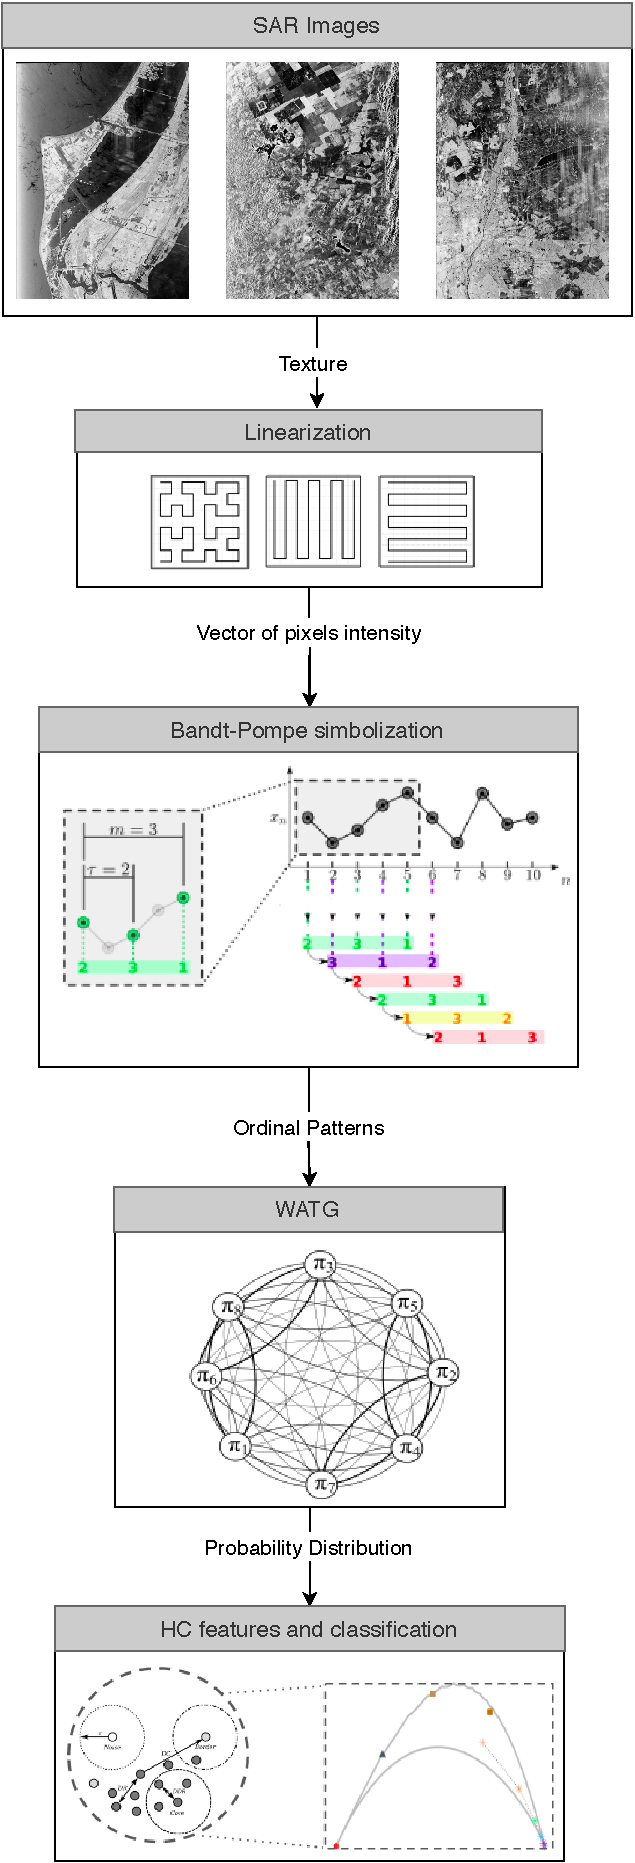
\includegraphics[scale = 0.7]{Figures/methodology.pdf}
	\caption{Outline of the methodology used for the classification of textures.}
	\label{fig:WATG}
\end{figure}

Our methodology consists of the following steps:
\begin{enumerate}
        \item \label{item:texture} extract the HHHH backscatter magnitudes of quad-polarimetric L-band SAR image, obtaining the image texture;
       \item\label{item:Linearlize} linearize a 2-D patch of data using the Hilbert-Peano curve;
        \item \label{item:Symbolization} employ the Bandt-Pompe symbolization to generate the set of ordinal patterns for each data sequence;
       \item\label{item:WOPTG} build the Ordinal Pattern Transition Graph with weighted edges to obtain a probability distribution function derived from this graph;
       \item\label{item:Descriptors} compute the Entropy and Statistical Complexity of this distribution and, finally, classify  regions.
\end{enumerate}
These steps are depicted in Fig.~\ref{fig:WATG}, and are detailed in the following.

\subsection{Linearization of image patches}\label{linearization}

In this step, we perform a data dimensionality reduction by turning 2-D patches into 1-D signals.
For this, we opt to do a linearization of the data through techniques that maintain the spatial correlation of the image.
This could be accomplished by reading the data by lines, columns, or any transformation.
In Step~\ref{item:Linearlize} we employ the Hilbert-Peano curve~\cite{Lee1994Texture}.

Nguyen et al.~\cite{nguyen1982space} firstly employed Space-filling curves,
%\todo[inline]{isso não era para ser uma citação?}
%DONE
to map texture into a one-dimensional signal.
When used as scanning methods of an image, such functions preserve relevant properties of pixel spatial correlation~\cite{Lee1994Texture}.

Carincotte et al.~\cite{UnsupervisedChangeDetectiononSARImagesUsingFuzzyHiddenMarkovChains} used the Hilbert-Peano curve in the problem of change detection in pairs of SAR images.
The authors noted that it exploits the spatial locality and that its pseudo-randomness
\todo[inline]{não entendi essa parte. pseudo-randomness of direction changes?}
 of direction changes works well for a large family of images, especially
natural ones.

Assuming an image patch is supported by a $N \times N$ dimension grid, where $N$ is a power of $2$, we have the following definition.

\newtheorem{mydef}{Definition}
\begin{mydef}
   An image scan is a bijective function $f \colon \mathbb{N} \times \mathbb{N} \to \mathbb{N}$ in the ordered pair set $ \{(i, j): 1 \leq i , j \leq N \}$, which denotes the points in the domain, for the closed range of integers $\{1, \dots, N^2\}$.
   A scan rule is $\{f^{-1}(1), \dots, f^{-1}(N^2)\}$.
   \label{def:CurveFilling}
\end{mydef}
This Definition imposes that each pixel is visited only once.

Space-filling curves, such as raster-1, raster-2, and Hilbert-Peano scanning techniques, stipulate a proper function $f$.
Hilbert-Peano curves scan an array of pixels of dimension $2^k \times 2^k$, $k \in \mathbb{N}$, never keeping the same direction for more than three consecutive points, as shown in Fig.~\ref{fig:Hilbert}.
Using the Hilbert-Peano curve, we can reduce the data dimensionality by maintaining the spatial dependence information of the analyzed textures.
In this work, we use only the Hilbert-Peano Curves scale in images of dimension $128 \times 128$.


\begin{figure}[hbt]
	\centering
	\tikz[scale=3.2] \hilbert((0mm,0mm),3);
	\hspace{0.3cm}
	\tikz[scale=1.5] \hilbert((0mm,0mm),4);
	\hspace{0.3cm}
	\tikz[scale=0.73] \hilbert((0mm,0mm),5);	
	\caption{Visual representation of Hilbert-Peano curve in areas of: (a) $8 \times 8$, (b) $16 \times 16$ and (c) $32 \times 32$. }\label{fig:Hilbert}
\end{figure} 

\subsection{Weighted Ordinal Patterns Transition Graph}\label{WATG}

Step~\ref{item:WOPTG} consists of two stages.
In the first, the time series is transformed into a sequence of ordinal patterns.
In the second, we build a weighted graph describing the transitions between these patterns.

The representation of time series by ordinal patterns was introduced by~\cite{Bandt2002Permutation} as a transformation resistant to noise, and invariant to nonlinear monotonic transformations.

Consider ${\mathcal X} \equiv \{x_t\}_{t=1}^{T}$ a real valued time series of length $T$. 

Let ${\mathfrak A}_{D}$ (with $D \geq 2$ and $D \in {\Bbb N}$) be the symmetric group of order $D!$ formed by all 
possible permutation of order $D$, and the symbol component vector 
${\bm \pi}^{(D)} = (\pi_1, \pi_2, \dots, \pi_D)$ so every element ${\bm \pi}^{(D)}$ is unique 
($\pi_j \neq \pi_k$ for every $j \neq k$). 
Consider for the time series ${\mathcal X} \equiv \{x_t\}_{t=1}^{T}$ its time delay embedding representation,
with embedding dimension $D \geq 2$ and time delay $\tau \geq 1$ ($\tau \in {\Bbb N}$, also called ``embedding time'', ``time delay'', or ``delay''):
\begin{equation} 
\label{eq:time-delay}
{\mathbf X}^{(D,\tau)}_t =( x_t,x_{t+\tau},\dots,x_{t+(D-1)\tau} ) ,
\end{equation} 
%
for $t = 1,2,\dots,N$ with $N = T-(D-1) \tau$.
Then the vector ${\mathbf X}^{(D,\tau)}_t$ can be mapped to a symbol vector ${\bm \pi}_t^D \in {\mathfrak A}_{D}$. 
This mapping should be defined in a way that preserves the desired relation between the elements 
$x_t  \in {\mathbf X}^{(D,\tau)}_t$, and all $t \in \{1,\dots,T-(D-1)\tau\}$ that share this pattern (also called ``motif'') have to be mapped to the same 
${\bm \pi}_t^{D}$.

We define the mapping ${\mathbf X}_t^{(D,\tau)} \mapsto {\mathbf \pi}_t^{D}$ by ordering the observations $x_t \in {\mathbf X}_t^{(D,\tau)}$ in increasing order.
Consider the time series $\mathcal X = (1.8, 1.2, 3.2, 4.8, 4.2, 4.5, 2.3, 3.7, 1.2, .5)$ depicted in Fig.~\ref{Fig:IntroBP}.
Assume we are using patterns of length $D=5$ with unitary time lag $\tau=1$.
The code associated to $\mathbf X_{3}^{(5,1)}=(x_3,\dots,x_7)=(3.2, 4.8, 4.2, 4.5, 2.3)$, shown in black, is formed by the indexes in $\bm\pi_3^{5}=(1,2,3,4,5)$ which sort the elements of $\mathbf X_{3}^{(5,1)}$ in increasing order: $51342$.
With this, $\widetilde{\pi}_3^{5} = 51342$, and we increase the counting related to this motif in the histogram of all possible patterns of size $D=5$.

The dash-dot line in Fig.~\ref{Fig:IntroBP} illustrates $\mathbf X_{1}^{(5,2)}$, i.e. the sequence of length $D=5$ starting at $x_1$ with lag $\tau=2$.
In this case, $\mathbf X_{1}^{(5,2)}= (1.8, 3.2, 4.2, 2.3, 1.2)$, and the corresponding motif is $\widetilde{\pi}_1^{5}=51423$.

\begin{figure}[hbt]
	\centering
	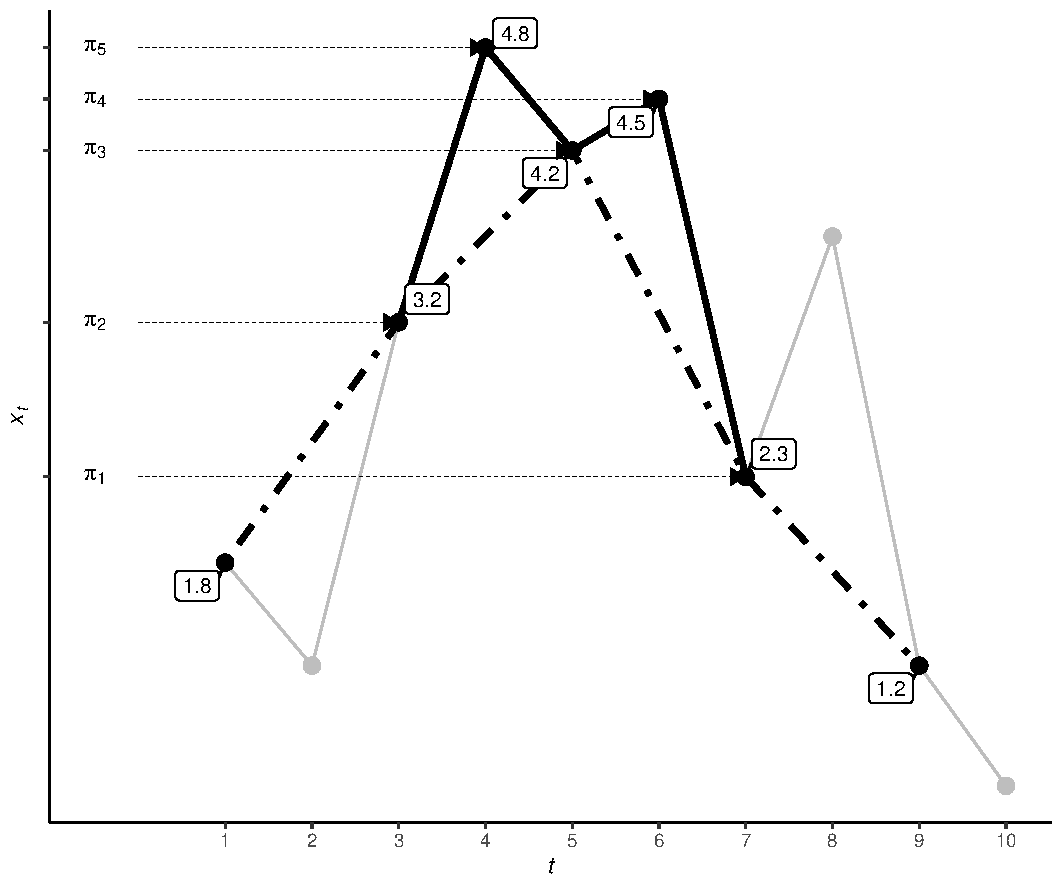
\includegraphics[width=.9\linewidth]{Figures/IntroBP.pdf}
	\caption{Illustration of the Bandt and Pompe coding\label{Fig:IntroBP}}
\end{figure}

The classical approach consists in analyzing the histogram of these patterns.
Alternatively, one may form an oriented graph with the transitions from $\widetilde\pi_t^D$ to $\widetilde\pi_{t+1}^D$. 
We modify this last approach by assigning weights to the edges related to the absolute difference of the observations.
This modification takes into account the scattering properties of the target, and leads to a good characterization of several types of textures.

Denote $\Pi$ the sequence of symbols obtained by a given series $\mathbf{X}_t^{(D,\tau)}$.
The Bandt-Pompe probability distribution is the relative frequency of symbols in the series against $D!$ possible permutations of patterns $\{\widetilde\pi_t^D \}_{t = 1}^{D!}$:
%\todo[inline]{Não sei como, mas essa equação tem que caber na largura da página. Sugestão:
%\begin{equation}
%   p(\widetilde\pi_t^D) = \frac{\#\left \{\mathbf{X}_t^{(D,\tau)} \text{ is of type } \widetilde\pi_t^D\right \}}{T- (D-1)\tau},  
%\end{equation}
%
%where  $t\in \{1, \dots, T-(D-1)\tau\}$.
%}
%DONE
%\begin{equation}
%p(\widetilde\pi_t^D) = \frac{\#\left \{t : t = 1, \dots, T-(D-1)\tau; \mathbf{X}_t^{(D,\tau)} \text{ is of type } \widetilde\pi_t^D\right \}}{T- (D-1)\tau},  
%\end{equation}
\begin{equation}
   p(\widetilde\pi_t^D) = \frac{\#\left \{\mathbf{X}_t^{(D,\tau)} \text{ is of type } \widetilde\pi_t^D\right \}}{T- (D-1)\tau},  
\end{equation}
where  $t\in \{1, \dots, T-(D-1)\tau\}$,that meets the conditions $p(\widetilde\pi_t^D) \ge 0$ and  $\sum_{i=1}^{D!} p(\widetilde\pi_t^D) = 1$.

The Ordinal Pattern Transition Graph ${G} = ({V}, {E})$ 
represents the transitions between two consecutive ordinal patterns over time $t$.
The vertices are the patterns, and the edges the transitions between them:
$V = \{v_{\widetilde\pi_t^D}\}$, and 
$E = \{(v_{\widetilde\pi_t^D}, v_{\widetilde\pi_{t+1}^D}): v_{\widetilde\pi_t^D}, v_{\widetilde\pi_{t+1}^D} \in V \}$~\cite{LearningandDistinguishingTimeSeriesDynamicsViaOrdinalPatternsTransitionGraphs2019}.

Recent works propose a weighting in the calculation of relative frequencies for ordinal patterns with different amplitude variances, making them contribute differently to the final value of the permutation entropy (PE) and thus incorporating amplitude change information within a given set~\cite{Fadlallah2013Weightedpermutation}.
However, these methods do not consider the amplitude difference present in different time series, weighing them similarly when calculating the final value of their probabilities.
Therefore, data with different amplitudes but with similar variance dynamics are not discriminated, losing important information about the system dynamics.

To counterbalance these facts, we propose a modification of the current ordinal pattern transition graph by incorporating meaningful time series information.

Two approaches are considered in relation to the weight of edges in the literature.
Some authors employ unweighted edge~\cite{McCullough2015lagged,Kulp2016ordinal} representing only the existence of such transitions, while others apply the frequency of transitions~\cite{Sorrentino2015periodic,Zhang2017ConstructingOP}.
The weights $\mathbb{W} = \{w_{v_{\widetilde{\pi}^D_i}, v_{\widetilde\pi^D_j}}: v_{\widetilde\pi^D_i}, v_{\widetilde\pi^D_j} \in V \}$ assigned to each edge describes the chance of transition between two particular patterns $(v_{\widetilde\pi^D_i}, v_{\widetilde\pi^D_j})$ calculated by their respective relative frequencies, ie:
\begin{equation}
w_{v_{\widetilde\pi^D_i}, v_{\widetilde\pi^D_j}} = \frac{|\Pi_{\widetilde\pi^D_i,\widetilde\pi^D_j}|}{T-(D-1)\tau-1},
\end{equation}
where $|\Pi_{\widetilde\pi^D_i,\widetilde\pi^D_j}|$ is the number of transitions from pattern $\widetilde\pi^D_i$ to pattern $\widetilde\pi^D_j$ and $\sum_{v_{\widetilde\pi^D_i}, v_{\widetilde\pi^D_j}}w_{v_{\widetilde\pi^D_i}, v_{\widetilde\pi^D_j}} = 1$,
and the denominator is the number of transitions between sequential patterns in the series of motifs of length $T-(D-1)\tau$.

Our proposal, henceforth referred to as Weighted Amplitude Transition Graph (WATG), incorporates the absolute difference between the observations that produced the patterns.


First, each $\mathcal{X}$ time series is scaled to $[0, 1]$, since we are interested in a metric able to compare datasets:
\begin{equation}
 \frac{x_i - x_{\min}}{x_{\max} - x_{\min}} \longmapsto x_i,
\end{equation}
where $x_{\min}$ and $x_{\max}$ are, respectively, the minimum and maximum values of the series.
This transformation is relatively stable before contamination, e.g., if instead of $x_{\max}$ we observe $k x_{\max}$ with $k\geq 1$, the relative values are not altered. Nevertheless, other more resistant transformations as, for instance, $z$ scores, might be considered.


Each $\mathbf{X}^{(D, \tau)}_t$ vector is associated with a weight $\beta_t$ that measures the largest difference between its elements:
\begin{equation}
\beta_t = \max\{x_i - x_j\},
\end{equation}
where $x_i, x_j \in \mathbf{X}^{(D, \tau)}_t$.

Traditionally, the transition graph assigns uniform weight to each transition between patterns and normalizes the result obtained by dividing by the total transitions.
In our proposal, %the $w_{v_{\widetilde\pi^D_i}, v_{\widetilde\pi^D_j}}$
 weights assigned to each edge depict the amplitude difference observed in the transition.
So we have that:	
\begin{equation}
w_{v_{\widetilde \pi^D_i}, v_{\widetilde \pi^D_j}} =  \sum_{i : \{\mathbf{X}^{(D,\tau)}_t \mapsto \widetilde\pi^D_i\}} \sum_{j : \{\mathbf{X}^{(D,\tau)}_t \mapsto \widetilde\pi^D_j\}} |\beta_i - \beta_j| .
\end{equation}
Thus, the probability distribution taken from the weighted amplitude transition graph is given as follows:	
\begin{align}
&\left\{\begin{array}{l}
\lambda_{v_{\widetilde\pi^D_i}, v_{\widetilde\pi^D_j}} = 1, \text{ if } (v_{\widetilde\pi^D_i}, v_{\widetilde\pi^D_j}) \in {E} \\
\lambda_{v_{\widetilde\pi^D_i}, v_{\widetilde\pi^D_j}} = 0, \text{ otherwise}.
\end{array}\right. \\
%
&p(\widetilde\pi^D_i, \widetilde\pi^D_j) = \frac{\lambda_{v_{\widetilde\pi^D_i}, v_{\widetilde\pi^D_j}} \cdot w_{v_{\widetilde\pi^D_i}, v_{\widetilde\pi^D_j}}}{\sum_{v_{\widetilde\pi^D_a}, v_{\widetilde\pi^D_b}} w_{v_{\widetilde\pi^D_a}, v_{\widetilde\pi^D_b}}}.
\end{align}

Note that the conditions $p(\widetilde\pi^D_i, \widetilde\pi^D_j) \ge 0$ and $\sum_{\widetilde\pi^D_i, \widetilde\pi^D_j} p(\widetilde\pi^D_i, \widetilde\pi^D_j) = 1$ are satisfied.

Thus, series with uniform amplitudes have edges with probability of occurrence well distributed along the graph, while those with large peaks have edges with probability of occurrence much higher than the others.

\subsection{Information-Theoretic Descriptors}\label{HC}

Entropy measures the disorder or unpredictability of a system characterized by a probability measure $\mathbb{P}$.

Let $\mathbb{P} = \{p_{(\widetilde\pi^D_1, \widetilde\pi^D_1)}, p_{(\widetilde\pi^D_1, \widetilde\pi^D_2)}, \dots, p_{(\widetilde\pi^D_{D!}, \widetilde\pi^D_{D!})} \} = \{p_1,\dots,p_{D!^2}\}$ be the probability distribution taken from the time series weighted amplitude transition graph $\mathbb{X}$.
The normalized Shannon entropy is given by:	
\begin{equation}
H(\mathbb{P}) = -\frac1{2\log D!}\sum_{\ell=1}^{D!^2} p_{\ell} \log p_{\ell} .
\label{eq:Entropia}
\end{equation}

The ability of the entropy to capture system properties is limited, so it is necessary to use it in conjunction with other des\-criptors to perform a more complete analysis.
Other interesting measures are distances between the $\mathbb{P}$ probability function and a probability measure that describes a non-informative process, typically the uniform distribution.

The Jensen-Shannon distance to the uniform distribution $\mathbb{U} = (\frac{1}{D!^2}, \dots, \frac{1}{D!^2})$ is a measure of how similar the underlying dynamics are to a process without information; it is calculated as:
\begin{equation}
Q'(\mathbb{P}, \mathbb{U}) = \sum_{\ell=1}^{D!^2} \Big(p_\ell \log\frac{p_\ell}{u_\ell} +
u_\ell \log\frac{u_\ell}{p_\ell}
\Big).
\end{equation}
This quantity is also called ``disequilibrium.''
The normalized disequilibrium is $ Q=Q'/\max\{Q'\}$.

Conversely to entropy, statistical complexity seeks to find interaction and dependence structures among the elements of a given series, being an extremely important factor in the study of dynamic systems.

The Statistical Complexity is then defined as~\cite{Lamberti2004}:
\begin{equation}
C(\mathbb{P}, \mathbb{U}) = H(\mathbb{P}) Q(\mathbb{P}, \mathbb{U}).
\end{equation}

In our analysis, each time series can then be described by a point $(H(\mathbb{P}), C(\mathbb{P}, \mathbb{U}))$.
The set of all pairs $(H(\mathbb{P}), C(\mathbb{P}, \mathbb{U}))$ for any time series described by patterns of length $D$ lies in a compact subset of $\mathbbm R^2$: the Entropy-Complexity plane. 

Through such a tool it is possible to discover the nature of the series, determining if it corresponds to a chaotic (or other deterministic dynamics) or stochastic sequences.

\section{EXPERIMENTAL RESULTS AND ANALYSIS}\label{Results}

In this section, we describe the dataset, the classification process and the results of the experiments.
To assess the performance of the developed technique, we first analyze the impact of its parameters and then compare its results generated in the classification with other methods.

\subsection{Image Dataset}

The proposed method was evaluated based on the HHHH backscatter magnitudes of three different quad-polarimetric L-band SAR images from the NASA Jet Propulsion Laboratory’s (JPL’s) uninhabited aerial vehicle synthetic aperture radar (UAVSAR):
\begin{itemize}
	\item Sierra del Lacandon National Park, Guatemala (acquired on April 10, 2015)\footnote{\protect{\url{https://uavsar.jpl.nasa.gov/cgi-bin/product.pl?jobName=Lacand_30202_15043_006_150410_L090_CX_01\#dados}}};
	\item Cape Canaveral Ocean Regions (acquired on September 22, 2016);
	\item Urban area of the city of Munich, Germany (acquired on June 5, 2015)\footnote{\protect{\url{https://uavsar.jpl.nasa.gov/cgi-bin/product.pl?jobName=munich_19417_15088_002_150605_L090_CX_01\#data}}}.
\end{itemize}

A total of $160$ uniform samples with size $128 \times 128$ were manually extracted from the images to compose the dataset used in the experiments, is organized as follows:
$40$ samples from Guatemalan forest regions;
$80$ samples from the oceanic regions of Cape Canaveral, where they were divided into two types that have distinct contrast information; and
$40$ samples of urban regions of the city of Munich.
Fig.~\ref{fig:example} a) shows examples of each of them.

Since the symbolization process is invariant to monotonous transformations and resistant to contamination effects, contrast changes are not capable of causing changes in the final results obtained by the descriptors.
Thus, the different types of oceanic regions considered in this work were studied as a single more general class.

In classification, to avoid overlap between training and validation samples, the data were divided into classes (regions of analysis) based on percentiles and random sampling occurs in each subgroup, preserving the general class distribution of the data.
Using this dataset, we have trained a K-nearest neighbor classifier algorithm with $85\%$ of all images and used tenfold cross-validation. 
The remaining $15\%$ of the images (that were never exposed to the learning algorithm) are used for testing the predictions.

\subsection{Analysis of ordinal patterns methods}

Fig.~\ref{fig:example} b) shows examples of the ocean, forest and urban samples as sequences values, after the linearization process.
\todo[inline]{Nessa figura 4B não seria interessante mostrar uma série temporal de cada tipo apresentado acima? Ou seja, uma de floresta, mar tipo 1 (seja lá que isso significa), mar tipo 2 (idem) e urbano?}
Data resulting from remote sensing have a peculiar feature that justifies the application in this article:
The variation in the magnitude of the targets' backscatter and, consequently, in the intensity of the image pixels, depends on the intrinsic properties of the regions under analysis.
Thus, urban targets are those that usually give the highest peaks, followed by forests, and finally, water bodies.
%\todo[inline]{ao invés dev falar em highest returns não seria melhor dizer "highest peaks?}
%DONE

By adding information related to the amplitude, the proposed method is able to capture important information from the signature of regions, presenting advantages in relation to the traditional methods of analysis of ordinal patterns.
\todo[inline]{Quais vantagens?}
In Fig.~\ref{fig:example} d), we can see the evolution of the descriptive power of these techniques.

As the first method in the literature for ordinal pattern analysis, the distribution of Bandt-Pompe calculated from the histogram of pattern frequencies manages to capture little information about the spatial structure of the textures, obtaining the worst result among the analyzed symbolization techniques. 
When considering the dynamics of alternating between consecutive patterns in a sequence, the transition graphs provide more information about the reference target and, consequently, this method is able to differentiate most of these dynamics, but there are challenging situations without a clear separation between them, causing misclassifications.
On the other hand, adding the magnitude of the pixel intensity in the calculation of the weights, we changed the priority of the transitions, increasing the importance of edges that represent the greatest amplitude variations along the sequence and decreasing (or erasing) the importance of others as it can be seen in Fig.~\ref{fig:example} c).\todo[inline]{Aqui precisa destacar no grafo o que acontece, ou seja, indicar as mudanças e quais os impactos delas no problema tratado.}
In this way, we were able to obtain, for this experiment, a perfect characterization and, consequently, the high descriptive power of the regions.

\begin{figure*}[!h]
	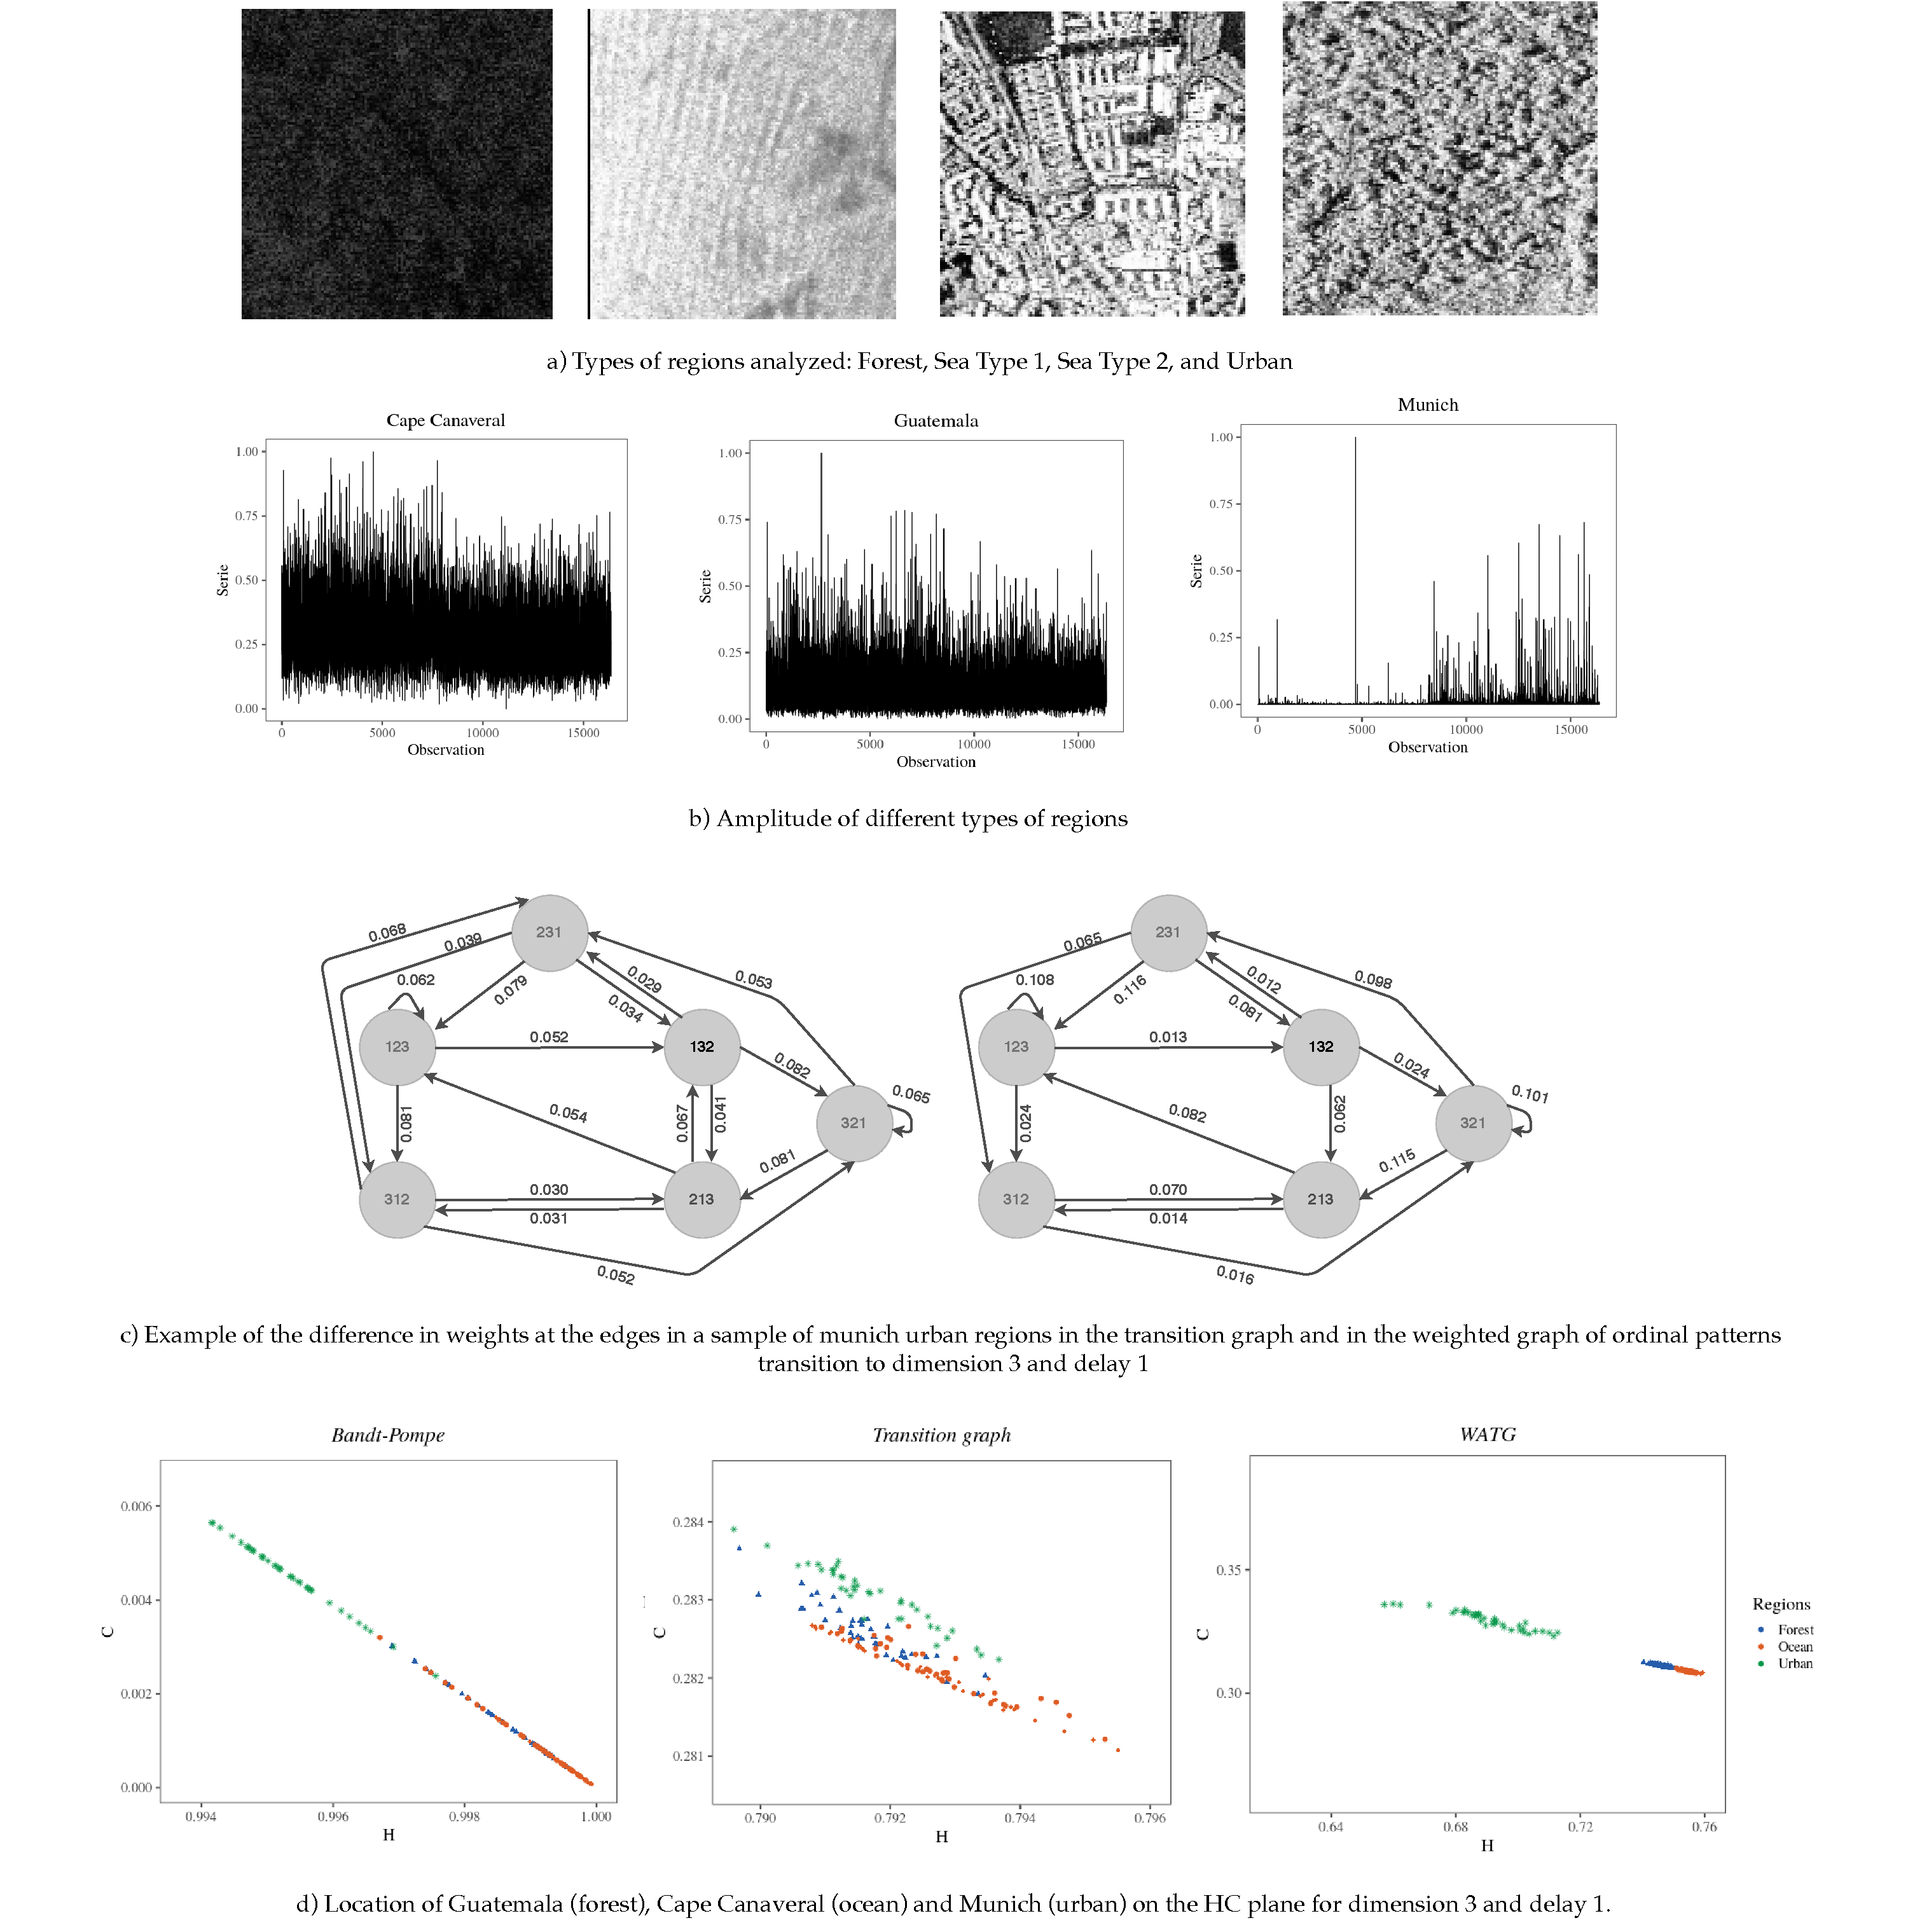
\includegraphics[width=2\columnwidth]{Figures/example.pdf}
	\caption{Main steps of the proposed method: 
	(1)~ Get samples of SAR texture images from different regions,
    (2)~ transform 2D image into a time series by linearization,
    (3)~ build the ordinal pattern transition graph to extract the distribution and
    (4)~ computing entropy and statistical complexity.}
	\label{fig:example}
\end{figure*}

\subsection{Experiments on sliding window selection}

\begin{figure}[h]
	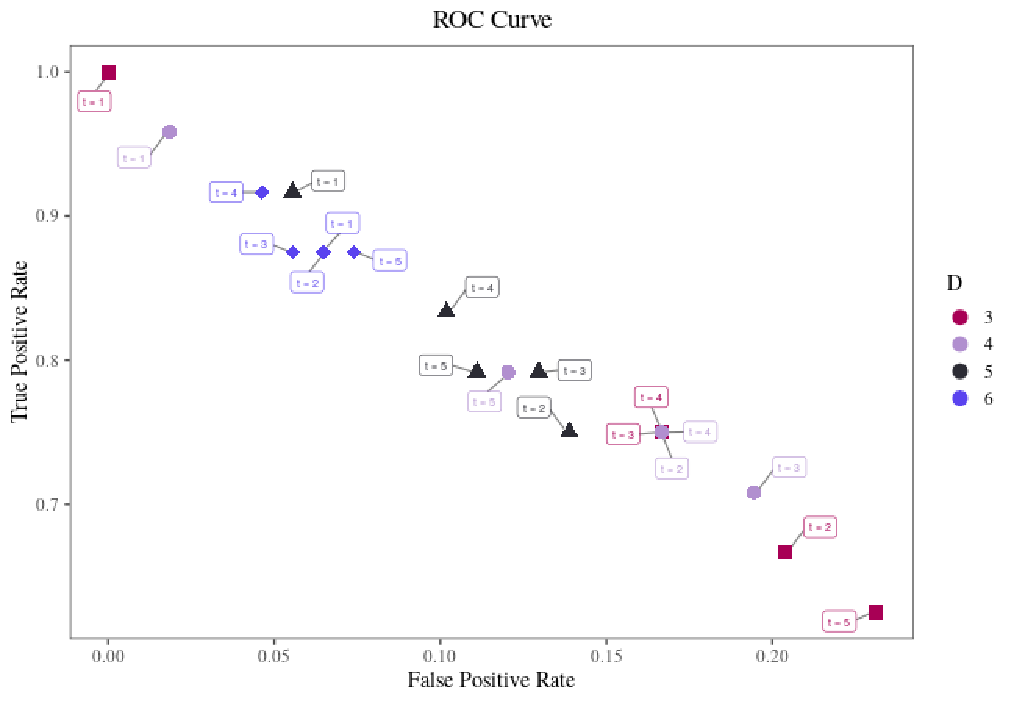
\includegraphics[width=\columnwidth]{Figures/ROC.pdf}	\caption{Evaluation of the sliding window parameters}
	\label{fig:ROC}
\end{figure} 

In this section, we analyze the parameters of the proposed method and its impact on the performance of the recognition of regions in textures, since inadequate values can hide important characteristics of the phenomenon under analysis~\cite{mccullough2015time}.
The two parameters of the transition graph modeling are: the dimension $D$, and the delay $\tau$.
In the experiments below, we present the results in the classification using different values of these parameters.

The performance of the classification method based on ordinal patterns is sensitive to the parameters of the sliding window used.
In transition graphs, as the size of the delay decreases, more patterns are produced, so we are able to capture more spatial dependencies between the elements and, consequently, more information about the dynamics of the system; therefore, it is expected that lower classification accuracy can be obtained with larger window size. \todo[inline]{acho que essa afirmação é bem forte, não teria que argumentar melhor? Para mim não ficou claro o fato de que mais padrões aparecem quando tau é menor. Tem referências para isso?}

To choose the most appropriate configuration of the sliding window parameters, we use the ROC curve shown in Fig.~\ref{fig:ROC} for different values of $D \in \{3, 4, 5, 6 \} $ and $\tau \in \{1, 2, 3, 4, 5 \}$.
This ROC was built as the rate of true positives versus the rate of false positives, with the one that comes closest to the $(0,1)$ point being selected as the best model.
The best model is reached when we keep the dimension and the delay in their smallest settings (i.e., $D = 3$ and $\tau = 1$), thus increasing the degree of information extracted from the series.\todo[inline]{aqui também eu não entendi porque D=3 e tau=1 garante que aumenta o nível de informação extraída. Tem que ter um certo cuidado com essas afirmações muito fortes. Tem referências para isso? Como podemos concluir isso apenas por essa análise? Talvez isso valha para esse experimento, se for isso, tem que ser melhor descrito}
Such an analysis also informs us that the best performance is acquired in the choice of parameters with the lowest computational cost.

We can observe, in Fig.~\ref{fig:Regions}, the spatial distribution of the points changes in relation to the parameters, allowing new grouping patterns to appear\todo[inline]{Não consegui ver novos grupos de padrões aparecendo. A figura não mostra os padrões, apenas os valores de HxC}.
When we apply small delay and dimension values with WATG, in urban region data, we obtained points with few extreme values, due to the typical peak values of their sequences. \todo[inline]{isso também não fica claro nessa figura, talvez fique na série temporal}
On the other hand, oceanic and forest regions have as their main discriminating descriptor the statistical complexity that portrays the degree of temporal dependence structure between the symbols and consequently between the pixel intensity values.

Fig.~\ref{fig:Regions} shows the characterizations for several dimension values $D$ and delays $\tau$.
Since such values inform us of intrinsic characteristics of the dynamics of the series in their specific domains, inadequate values may hide this kind of knowledge about the data, and this analysis step is crucial.

As shown in Fig.~\ref{fig:Regions}, class discrimination decreases with increasing $\tau$, which means that there is a loss of effect from the variation of pixels values in the series, thus making a better distinction between classes when we have $\tau = 1$.\todo[inline]{Isso não estaria relacionado ao fato de que valores maiores de tau faria com que se perdesse a estrutura de dependência espacial pois os pontos vizinhos na amostra tendem a ficar mais distantes na imagem?}
As WATG captures amplitude differences between different time series, when the values of the $\tau$ scale increase, well-distributed weight plots are formed, thus obtaining increasing entropy values.
On the other hand, as we increase $D$, the granularity of the information increases, capturing more spatial dependence structures in the data and, consequently, acquiring greater statistical complexity.
There is a relationship between the dimension variable of ordinal patterns and the discrimination between the analyzed regions that presents its best result for $D = 3$.
On the other hand, when we have $D = 6$, textures acquire a lower entropy value and become harder to distinguish.
\todo[inline]{Acho que é bom usar transparência nos pontos para a gente perceber que tem sobreposição de classes em alguns casos eque D=3 de Tau=1 é a configuração que separa melhor as classes}
\begin{sidewaysfigure*}
	\centering
	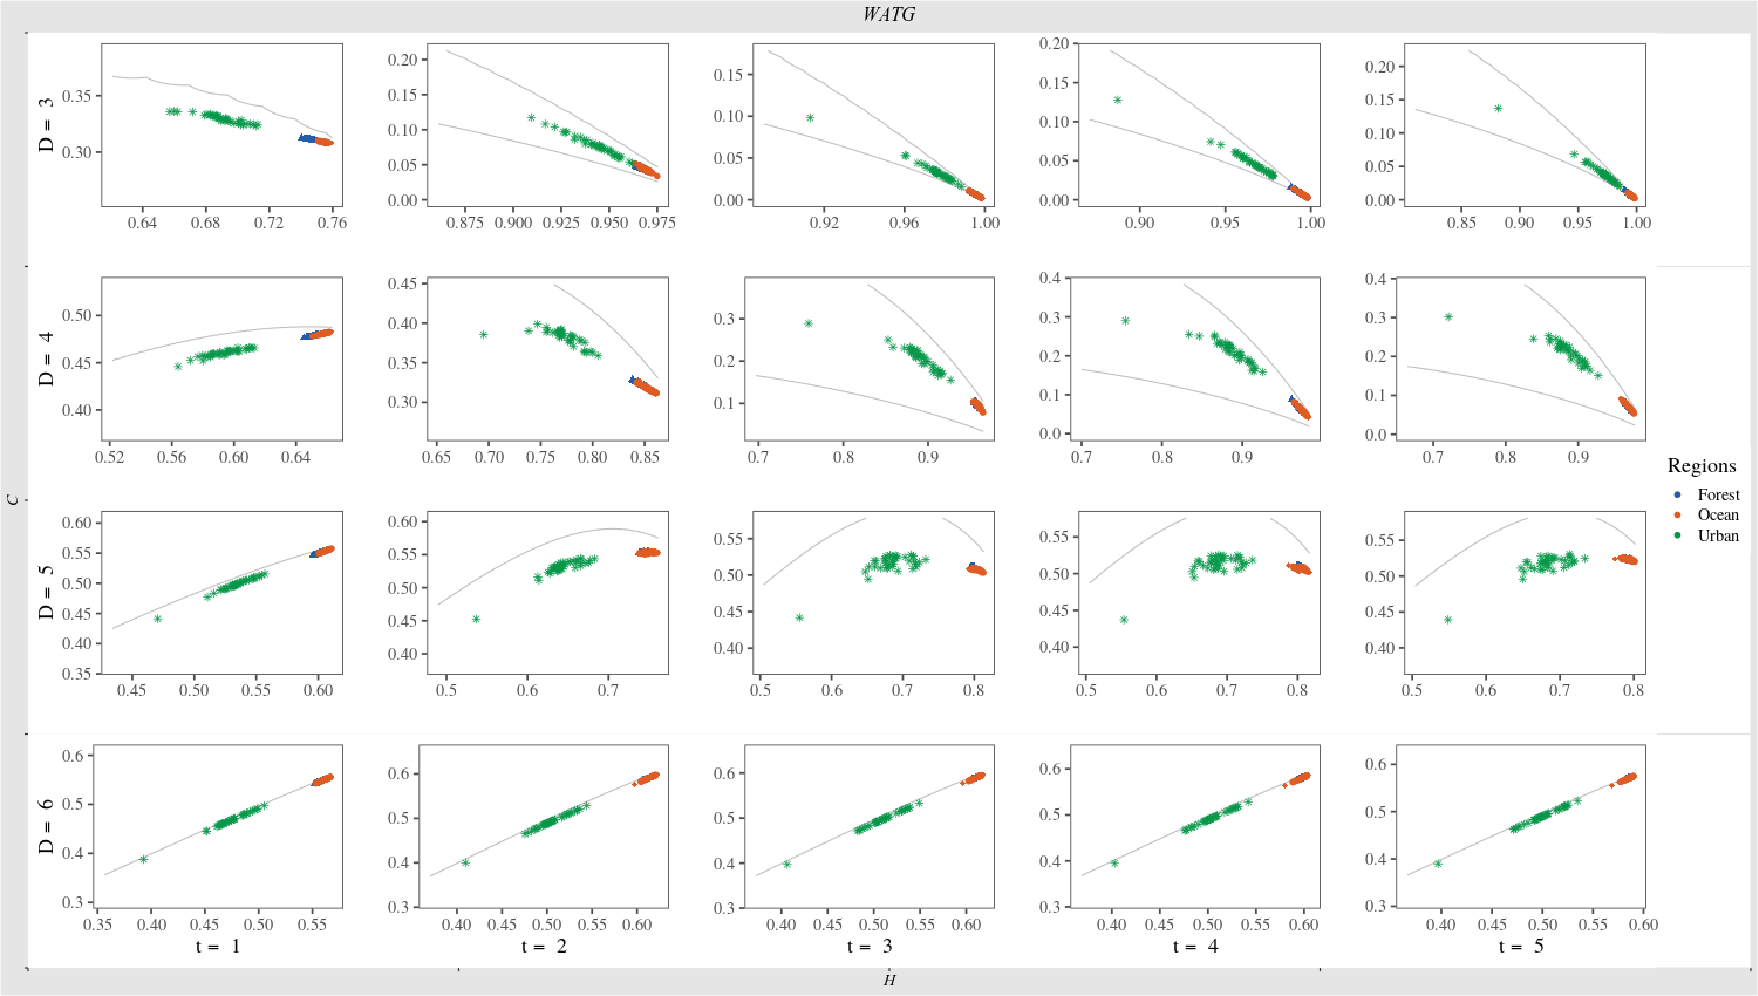
\includegraphics[width=1\textwidth]{Figures/WATGHC.pdf}
	\caption{Characterization resulting in HC Plane from the application of the Hilbert-Peano curve in WATG on textures of different regions: Guatemala (forest), Cape Canaveral (ocean) and Munich (urban).}
	\label{fig:Regions}
\end{sidewaysfigure*}

\subsection{Quantitative Evaluation}

Several experiments were carried out to validate the features extracted from the information theory descriptors in the characterization and classification of regions.
In this subsection, we present a comparison between the proposed method and other methods present in the literature for characterization with ordinal patterns and texture classification.
In the comparisons, we use the following four methods: gray level co-occurrence matrices~\cite{kourgli2012texture}, Gabor filters~\cite{weldon1996efficient}, Bandt-Pompe probability distribution~\cite{Bandt2002Permutation}, and ordinal patterns transition graph~\cite{borges2019learning}.
For each co-occurrence matrix, four statistics are selected: contrast, correlation, energy, and homogeneity.
Gabor filters are implemented in five scales and eight orientations and the energy is used as a feature. 
An 80-dimensional feature vector was obtained for each patch.
We consider the traditional implementation of each method.\todo[inline]{Referências para os métodos são super bem-vindas aqui}

To evidence the importance of features in the classification process, we chose the algorithm of the k-nearest neighbors, due to its simplicity.
In all experiments, we used Euclidean distance and 10 resampling interactions and a 10-fold cross-validation method to evaluate our proposal.
%\todo[inline]{Essa frase não seria melhor se fosse apenas "we used a 10-fold cross-validation method to assess our proposal? Algo assim?}
%DONE
More details about the classifier and the sampling scheme can be seen in~\cite{mitchell1997machine}. 

In addition, the automatic grid search method of the Caret R package is applied to estimate the k parameter of the k-nearest neighbors algorithm~\cite{kuhn2008building}.
This can be done by configuring the tuneLength parameter of the train function to sample a certain number of candidates from a hyper-parameter.
The following results demonstrate the automatic grid search of the KNN attribute k with 20 (tuneLength = 20) attempts of values (20 total models).

The experimental results of the 160 samples of the dataset used are presented in the Table~\ref{tab:result1}.
We assess the effectiveness of each approach using the following metrics: recall or true positive rate (TPR), precision or positive predictive value (PPV), overall accuracy (OA), and F1-score.

As expected, we can see that the result obtained by the Bandt-Pompe distribution reached the lowest results with OA $= 70.8\%$ and F1-score $= 22.2\%$.
Then, we followed the improvement in the descriptive power of ordinal patterns with the transition graph that obtained OA $= 83.3\%$ and F1-score $= 60.0\%$.
We can also observe that GLCM is not able to have high descriptive power in the proposed dataset, obtaining OA $= 66.6\%$ and F1-score $= 80.0\%$.
In addition, it is observed that the highest success rate was obtained by the proposed method, which provided results comparable to the Gabor filters that acquired OA $= 100\%$ and F1-score $= 100\%$.
Thus, when applying WATG we managed to maintain the success rate using fewer features and, consequently, less computational power since only two descriptors were used in the characterization. {\color{red}Our method is also less susceptible to the so-called curse of the dimensionality when compared to the use of Gabor Filters.}

\begin{table*}[!h]
\centering
\caption{Experimental results using KNN}
\label{tab:result1}
\begin{tabular}{|l|l|lll|lll|l|l|}
\hline
Method      & N. of features         &       & TPR   &       &       & PPV    &       & OA  & F1-Score \\ \cline{3-8} 
                 &   & Urban & Forest & Ocean & Urban & Forest & Ocean & &  \\\hline
Bandt-Pompe HC   & 2 & 0.833 &  0.666  & 0.833 & 1.000 & 0.571  & 0.833 & 0.792 &  0.615  \\ 
Transition Graph HC & 2  & 1.000 & 0.666  & 0.916 & 0.857 & 1.000  & 0.846 & 0.875 & 0.800 \\
WATG HC         & 2  & 1.000 & 1.000  & 1.000 & 1.000 & 1.000  & 1.000 & 1.000 & 1.000 \\ 
Gabor           & 80  & 1.000 & 1.000  & 1.000 & 1.000 & 1.000  & 1.000 & 1.000 & 1.000\\
GLCM            & 4   & 1.000 & 0.833  & 1.000 & 1.000 & 1.000  & 0.923 & 0.666 & 0.800\\
\hline
\end{tabular}
\end{table*}

\section{CONCLUSION}\label{Conclusion}

In the study presented, a new method of analysis and classification of SAR images was presented.
This method consists of three steps, the linearization of the SAR image texture, the weighted ordinal pattern transition graph technique, based on the Bandt-Pompe symbolization method, and the information theory descriptors.

The main objective of the proposed method is to find a probability distribution of ordinal patterns sensitive to amplitude information and that, due to the backscattering properties of the SAR image sensors, classifies different regions of analysis.
Detection and classification were performed using the k-nearest neighbors algorithm of supervised learning.
Experiments with UAVSAR images demonstrated that the proposal meets a performance superior to that of competing methods and similar to the Gabor filter.
However, when applied, it overcomes some disadvantages of the Gabor filter, managing to maintain its effectiveness in classifying different regions in SAR image textures.
For example, it does not need a large number of features and therefore a high computational power.

As a result, in addition to perfectly separating urban areas from the others analyzed by entropy values, we are still able to differentiate oceanic and forest areas through their different values of statistical complexity, which informs us of the degree of spatial dependence between their elements.
The proposed method is also invariant to monotonous transformations and resistant to the effects of contamination, even changes, in contrast, do not cause changes in the descriptors of the images.
In the future, we hope to continue to refine the extraction of texture features, proposing an extension of the algorithm for the segmentation of regions and investigate the effects of their use in other applications e.g., erosion monitoring and urban activities.

\section{SOURCE CODE AVAILABILITY} 

%\todo{Atualizar o repositório}

The source code generated during the current study are available in the \textit{SAR-WATG} repository, \url{https://github.com/EduardaChagas/SAR-WATG}.

\bibliographystyle{IEEEtran}
\bibliography{../../Common/sar.bib}

\section*{ACKNOWLEDGEMENTS}\label{ACKNOWLEDGEMENTS}

This work was partially funded by the Coordination for the Improvement of Higher Education Personnel (CAPES) and National Council for Scientific and Technological Development (CNPq).

\end{document}  